\chapter{Principal component analysis}
\minitoc
\begin{kwd}
Principal components; singular value decomposition.
\end{kwd}

Principal component analysis is a multivariate technique which aims at analyzing the statistical structure of high dimensional dependent observations by representing data using orthogonal variables called {\em principal components}. Its origin may be traced back to \cite{hotelling:33} who first introduced the principal components as a way to reduce the dimensionality of the data. Reducing the dimensionality of the data is motivated by several practical reasons such as improving computational complexity.

Let $(X_i)_{1\leqslant i\leqslant n}$ be i.i.d. random variables in $\rset^d$ and consider the matrix $X\in\rset^{n\times d}$ such that the $i$-th row of $X$ is the observation $X^\top_i$. In this chapter, it is assumed that data are preprocessed so that the columns of $X$ are centered ($X$ is replaced by $X - n^{-1}\mathbf{1}^\top_n\ones_nX$ if the columns of $X$ are not centered).  This means that for all $1\leqslant j \leqslant d$, $\sum_{i=1}^{n}X_{i,j} = 0$. Let $\Sigma_n$ be the empirical covariance matrix:
$$
\Sigma_n = n^{-1}\sum_{i=1}^n X_i X^\top_i\eqsp.
$$

Principal Component Analysis  aims at reducing the dimensionality of the observations $(X_i)_{1\leqslant i \leqslant n}$ using a {\em compression} matrix $W\in \rset^{p\times d}$ with $1\leqslant p\leqslant d$ so that for each $1\leqslant i \leqslant n$, $WX_i$ is a low dimensional representation of $X_i$. The original observation may then be partially recovered using another matrix $U\in \rset^{d\times p}$. Principal Component Analysis  computes $U$ and $W$ using the least squares approach:
\begin{align*}
(U_{\star},W_{\star}) \in \hspace{-0.5cm}\underset{(U,W)\in \rset^{d\times p}\times \rset^{p\times d}}{\mathrm{argmin}} \;\sum_{i=1}^n\|X_i - UWX_i\|_2^2\eqsp.
\end{align*}

%The source codes in R and/or Python of this chapter may be found at:
%\[
%\mathrm{https\!:\!\!/\!/sylvainlecorff.github.io/algorithms}
%\]


\section{Principal Component Analysis as a singular value decomposition problem}
\label{sec:pca:svd}
\subsection{Singular value decomposition}

\begin{shaded}
\begin{proposition} 
\label{prop:acp:svd}
For all $\rset^{n \times d}$ matrix $A$ with rank $r$, there exist $\sigma_1\geqslant \ldots \geqslant \sigma_r>0$ such that
\[
A = \sum_{k=1}^r \sigma_k u_k v^\top_k\eqsp,
\]
where $\{u_1,\ldots,u_r\}\in (\rset^n)^r$ and $\{v_1,\ldots,v_r\}\in (\rset^d)^r$ are two orthonormal families. The vectors $\{\sigma_1,\ldots,\sigma_r\}$ are called singular values of $A$ and $\{u_1,\ldots,u_r\}$ (resp. $\{v_1,\ldots,v_r\}$) are the left-singular (resp. right-singular) vectors of $A$.
\end{proposition}
\end{shaded}
\begin{remark}
If $U$ denotes the $\rset^{n\times r}$ matrix with columns given by $\{u_1,\ldots,u_r\}$ and $V$ denotes the $\rset^{p \times r}$ matrix with columns given by $\{v_1,\ldots,v_r\}$, then the singular value decomposition of $A$ may also be written as
\[
A = UD_rV^\top\eqsp,
\]
where $D_r = \diag(\sigma_1,\ldots,\sigma_r)$.
\end{remark}
\begin{remark}
The singular value decomposition is closely related to the spectral theorem for symmetric semipositive definite matrices. In the framework of Proposition~\ref{prop:acp:svd}, $A^\top A$ and $AA^\top$ are positive semidefinite such that
\[
A^\top A = VD_r^2V^\top\quad\mathrm{and}\quad AA^\top = UD_r^2U^\top\eqsp.
\]
\end{remark}
\begin{proof}
Since the matrix $AA^\top$ is positive semidefinite, its spectral decomposition is given by
\[
AA^\top = \sum_{k=1}^r \lambda_k u_k u^\top_k\eqsp,
\]
where $\lambda_1\geqslant \ldots\geqslant \lambda_r>0$ are the nonzero eigenvalues of $AA^\top$ and $\{u_1,\ldots,u_r\}$ is an orthonormal family of $\rset^n$. For all $1\leqslant k\leqslant r$, define $v_k = \lambda_k^{-1/2}A^\top u_k$ so that
\begin{align*}
\|v_k\|^2&=\lambda_k^{-1}\langle A^\top u_k;A^\top u_k\rangle = \lambda_k^{-1} u_k^\top AA^\top u_k = 1\eqsp, \\
A^\top Av_k & = \lambda_k^{-1/2}A^\top A A^\top u_k  = \lambda_k v_k\eqsp.
\end{align*}
On the other hand, for all $1\leqslant k\neq j\leqslant r$, $\langle v_k;v_j\rangle = \lambda_k^{-1/2}\lambda_j^{-1/2}u^\top_kA A^\top u_j =\lambda_k^{-1/2}\lambda_j^{1/2}u^\top_ku_j = 0$. Therefore, $\{v_1,\ldots,v_r\}$ is an orthonormal family of eigenvector of $A^\top A$ associated with the eigenvalues $\lambda_1\geqslant \ldots\geqslant \lambda_r>0$. 
Define, for all $1\leqslant k\leqslant r$, $\sigma_k = \lambda_k^{1/2}$ which yields
\[
\sum_{k=1}^r \sigma_k u_k v^\top_k = \sum_{k=1}^r  u_k u^\top_kA = \left(\sum_{k=1}^r  u_k u^\top_k\right)A\eqsp.
\]
As $\{u_1,\ldots,u_r\}$ is an orthonormal family, by Lemma~\ref{lem:ortho:proj}, $UU^\top = \sum_{k=1}^r u_ku^\top_k$ is the orthogonal projection onto the $\mathrm{range}(AA^\top) = \mathrm{range}(A)$ which implies
\[
\sum_{k=1}^r \sigma_k u_k v^\top_k = \left(\sum_{k=1}^r  u_k u^\top_k\right)A = A\eqsp.
\]
\end{proof}
An illustration of SVD is given in Figure~\ref{fig:svd:rec}. In this setting, the matrix $A$ is a 848 $\times$ 1280 matrix of grayscale pixels. 
\begin{figure*}
        \centering
            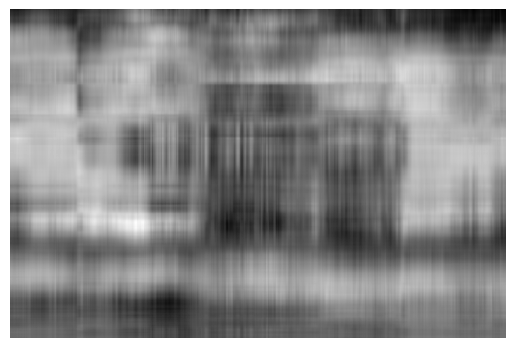
\includegraphics[width=.45\textwidth]{./Illustrations/svd_5}
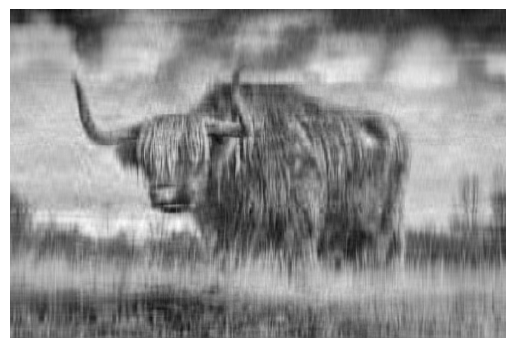
\includegraphics[width=.45\textwidth]{./Illustrations/svd_25}
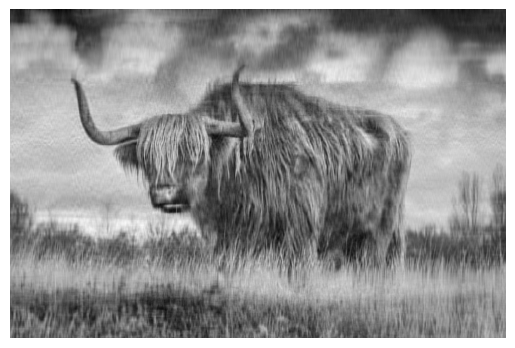
\includegraphics[width=.45\textwidth]{./Illustrations/svd_50}
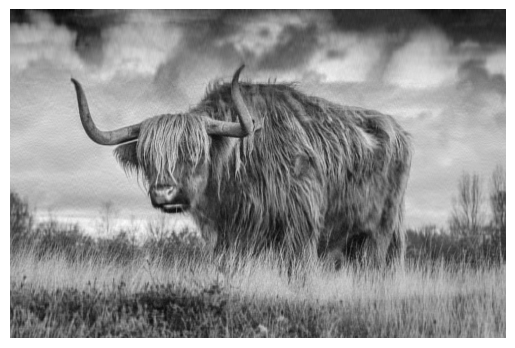
\includegraphics[width=.45\textwidth]{./Illustrations/svd_100}
        \caption{\small Image reconstruction using  the largest singular values of the SVD. The original grayscale image (from \url{https://pixabay.com/}) is given by a matrix ox pixels of size 848 $\times$ 1280. Reconstruction given with the top 5 (top left), 25 (top right), 50 (bottom left) and 100 (bottom right) singular values.} 
        \label{fig:svd:rec}
    \end{figure*}
\begin{figure*}
        \centering
            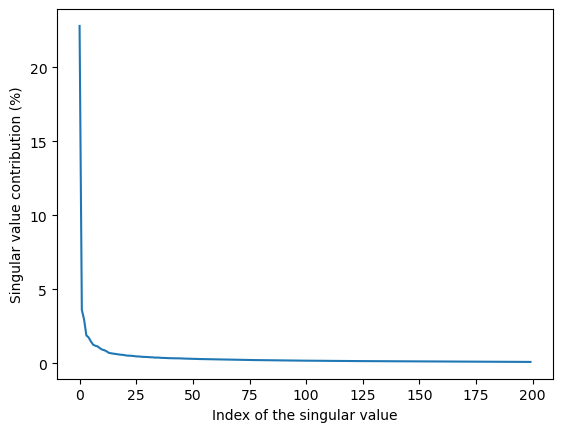
\includegraphics[width=.60\textwidth]{./Illustrations/svd_sv}
        \caption{\small Singular value contributions: for all $1\leqslant i \leqslant 200$, the contribution of $\sigma_i$ is given by $\sigma_i/(\sum_{j=1}^{200}\sigma_j)$.} 
        \label{fig:svd:sv}
    \end{figure*}
%\includepdf[pages=-]{./Data/svd_image_compression.pdf}

\subsection{Application to Principal Component Analysis}
As mentioned in the introduction, Principal Component Analysis aims at solving the following optimization problem:
\begin{align}
\label{eq:pca:uw}
(U_{\star},W_{\star}) \in \hspace{-0.5cm}\underset{(U,W)\in \rset^{d\times p}\times \rset^{p\times d}}{\mathrm{argmin}} \;\sum_{i=1}^n\|X_i - UWX_i\|_2^2\eqsp.
\end{align}

\begin{shaded}
\begin{lemma} 
\label{lem:acp:ortho}
Let $(U_{\star},W_{\star})\in \rset^{d\times p}\times \rset^{p\times d}$ be a solution to \eqref{eq:pca:uw}. Then, the columns of $U_{\star}$ are orthonormal and $W_{\star} = U^\top_{\star}$.
\end{lemma}
\end{shaded}
%\begin{proof}
%To be added.
%\end{proof}
Let $U\in\rset^{d\times p}$ be such that $U^\top U = \Id_p$. Then,
\begin{align*}
\sum_{i=1}^n\|X_i - UU^\top X_i\|_2^2 &= \sum_{i=1}^n\|X_i\|_2^2 + \sum_{i=1}^n\|UU^\top X_i\|_2^2 - 2\sum_{i=1}^n\langle X_i;UU^\top X_i\rangle\eqsp,\\
&=  \sum_{i=1}^n\|X_i\|_2^2 + \sum_{i=1}^nX^\top_iUU^\top X_i - 2\sum_{i=1}^nX^\top_iUU^\top X_i\eqsp,\\
&=  \sum_{i=1}^n\|X_i\|_2^2 - \sum_{i=1}^nX^\top_iUU^\top X_i\eqsp,\\
&=  \sum_{i=1}^n\|X_i\|_2^2 - \sum_{i=1}^n\mathrm{trace}(U^\top X_iX_i^\top U)\eqsp.
\end{align*}
Therefore, by Lemma~\ref{lem:acp:ortho}, solving \eqref{eq:pca:uw} boils down to computing
\begin{align}
\label{eq:pca:u}
U_{\star} \in \hspace{-0.5cm}\underset{U\in \rset^{d\times p}\eqsp,\eqsp U^\top U = \Id_n}{\mathrm{argmax}} \hspace{-.4cm}\{ \mathrm{trace}(U^\top\Sigma_nU)\}\eqsp.
\end{align}


\begin{shaded}
\begin{proposition} 
\label{prop:acp:svd}
Let $\{\vartheta_1,\ldots,\vartheta_d\}$ be orthonormal eigenvectors associated with the eigenvalues $\lambda_1\geqslant \ldots \geqslant \lambda_d$ of $\Sigma_n$. Then a solution to \eqref{eq:pca:uw} is given by the matrix $U_{\star}$ with columns $\{\vartheta_1,\ldots,\vartheta_p\}$ and $W_{\star} = U^\top_{\star}$.
\end{proposition}
\end{shaded}
\begin{proof}
By Lemma~\ref{lem:acp:ortho} and \eqref{eq:pca:u}, the proof is equivalent to prove that $U_{\star}$ is a solution to \eqref{eq:pca:u}. Let $\Sigma_n = VD_nV^\top$ be the spectral decomposition of $\Sigma_n$ where $D_n = \diag(\lambda_1,\ldots,\lambda_d)$ and $V\in\rset^{d\times d}$  is a matrix with columns $\{\vartheta_1,\ldots,\vartheta_d\}$. For all  matrix $U\in\rset^{d\times p}$  with orthonormal colums define $B = V^\top U$ so that, as $V\in\rset^{d\times d}$ is an orthogonal matrix,  
\[
VB = VV^\top U = U\quad\mathrm{and}\quad U^\top\Sigma_n U = B^\top V^\top VD_nV^\top VB = B^\top D_nB\eqsp.
\] 
Therefore,
\begin{equation}
\label{eq:pca:trace}
\mathrm{Trace}(U^\top\Sigma_n U) = \mathrm{Trace}(B^\top D_nB) = \sum_{i = 1}^d \lambda_i \sum_{j=1}^p b^2_{i,j}\eqsp.
\end{equation}
On the other hand,
\[
B^\top B = U^\top VV^\top U = U^\top U = \Id_p\eqsp,
\]
so that the columns of $B$ are orthonormal and
\[
\sum_{i = 1}^d \sum_{j=1}^p b^2_{i,j} = p\eqsp.
\]
% Therefore, for all $1\leqslant j,k \leqslant p$, $\sum_{i=1}^d\vartheta_i U_jU_k'\vartheta_i=\delta_{j,k}$ which yields, for all $1\leqslant j\leqslant p$, 
%\[
%\sum_{i=1}^d\vartheta_i' U_jU_j'\vartheta_i= 1\eqsp.
%\]
%Then,
%\[
%\sum_{j=1}^p b^2_{i,j} = \sum_{j=1}^p(\vartheta_i' U_j)^2 = \sum_{j=1}^p\vartheta_i' U_jU_j'\vartheta_i
%\]
%and, by \eqref{eq:pca:trace},
%\[
%\mathrm{Trace}(U'\Sigma_n U) \leqslant \sum_{i = 1}^p \lambda_i \eqsp.
%\]
%
%
By \eqref{eq:pca:trace},
\[
\mathrm{Trace}(U^\top\Sigma_n U) = \sum_{i=1}^{d}\alpha_i\lambda_i\eqsp,
\]
with, for all $1\leqslant i\leqslant d$, $\alpha_i \in[0,1]$ and $\sum_{i=1}^d\alpha_i  = p$. As $\lambda_1 \geqslant \lambda_2\geqslant \ldots, \lambda_d$\eqsp,
\[
\mathrm{Trace}(U^\top\Sigma_n U) \leqslant \sum_{i=1}^{p}\lambda_i\eqsp.
\]
As the columns of $U_{\star}$ are$\{\vartheta_1,\ldots,\vartheta_p\}$, for all $1\leqslant i\leqslant d$ and $1\leqslant j \leqslant p$, $b_{i,j} = \langle \vartheta_i;\vartheta_j\rangle = \delta_{i,j}$. Therefore,  for all $1\leqslant i\leqslant d$, $\sum_{j=1}^p b^2_{i,j} = 1$ and by \eqref{eq:pca:trace},
\[
\mathrm{Trace}(U_{\star}^\top\Sigma_n U_{\star}) =\sum_{i = 1}^p \lambda_i\eqsp,
\]
which completes the proof.
\end{proof}

\section{Principal Component Analysis: projection onto a subspace}
 For any dimension $1\leqslant p \leqslant  d$, let $\calF_d^p$ be the set of all vector suspaces of $\rset^d$ with dimension $p$. In this section, it is proved that  Principal Component Analysis computes a linear span $V_d$ such as
\begin{align}
\label{eq:pca:proj}
V_p \in \underset{V\in \calF_d^p}{\mathrm{argmin}} \;\sum_{i=1}^n\|X_i - \pi_V(X_i)\|_2^2\eqsp, 
\end{align}
where $\pi_V$ is the orthogonal projection onto the linear span $V$.
Assume first that $p = 1$ and write $V_1 = \mathrm{span}\{v_1\}$ for $v_1\in \rset^d$ such that $\|v_1\|_2 = 1$. Then, 
\begin{align*}
\sum_{i=1}^n\|X_i - \pi_{V_1}(X_i)\|_2^2 & = \sum_{i=1}^n\|X_i -  \langle X_i; v_1 \rangle v_1 \|_2^2\eqsp,\\
& = \sum_{i=1}^n \left( \|X_i\|_2^2 - 2 \langle X_i; \langle X_i; v_1 \rangle v_1 \rangle + \| \langle X_i; v_1 \rangle v_1 \|_2^2 \right)\eqsp,\\
& = \sum_{i=1}^n \left( \|X_i\|_2^2 -   \langle X_i; v_1 \rangle^2 \right).
\end{align*}
Consequently, $V_1$ is a solution to \eqref{eq:pca:proj} if and only if $v_1$ is solution to:
\[
v_1 \in \underset{v \in \rset^d\,;\, \|v\|_2=1}{\mathrm{argmax}} \sum_{i=1}^n   \langle X_i, v \rangle^2\eqsp.
\]
For all $2\leqslant p \leqslant d$, following the same steps, it can be proved that  a solution to \eqref{eq:pca:proj} is given by $V_p = \mathrm{span}\{v_1, \ldots, v_p\}$ where
\begin{equation}
\label{eq:vecpca}
v_1 \in \underset{v\in \rset^d\,;\,\|v\|_2=1}{\mathrm{argmax}} \sum_{i=1}^n\langle X_i,v\rangle^2 \quad\mbox{and for all}\;\; 2\leqslant k \leqslant p\;,\;\; v_k \in \underset{\substack{v\in \rset^d\,;\,\|v\|_2=1\,;\\ v\perp v_1,\ldots,v\perp v_{k-1}}}{\mathrm{argmax}}\sum_{i=1}^n\langle X_i,v\rangle^2\eqsp. 
\end{equation}
%To prove the general formula, just note that, letting $V_d = \mathrm{span}\{v_1, \hdots, v_d\}$, and $\tilde V_{d-1} = 	\mathrm{span}\{v_2, \hdots, v_d\}$,
%\begin{align*}
%\sum_{i=1}^n\|x_i - \pi_{V_d}(x_i)\|^2 & = \sum_{i=1}^n\| (x_i - \pi_{\tilde V_{d-1}}(x_i) ) - \pi_{v_1}(x_i - \pi_{\tilde V_{d-1}}(x_i) ) \|^2\eqsp.
%\end{align*}
%With the same arguments as above, for all $v_2, \hdots, v_d$, 
%\begin{align*}
%v_1 \in \underset{\substack{v_1 \in \R^p\,;\\\, \|v_1\|=1\,;\\}}{\mathrm{argmax}} \sum_{i=1}^n   \langle x_i - \pi_{\tilde V_{d-1}}(x_i), v_1 \rangle^2,
%\end{align*}
%which is equivalent to 
%\begin{align*}
%v_1 \in \underset{\substack{v_1 \in \R^p\,;\\\, \|v_1\|=1\,;\\}}{\mathrm{argmax}} \sum_{i=1}^n   \langle x_i - \pi_{\tilde V_{d-1}}(x_i), v_1 \rangle^2 = \sum_{i=1}^n   \langle x_i, v_1 \rangle^2\eqsp.
%\end{align*}
%The other formula can be proved in the exact same manner. 
%\subsection*{Principal Component Analysis as a singular value decomposition}
It remains to prove that the vectors $\{v_1, \ldots , v_k\}$ defined by \eqref{eq:vecpca} can be chosen as the orthonormal eigenvectors associated with the $k$ largest eigenvalues of the empirical covariance matrix $\Sigma_n$. Note that for all $v\in \rset^d$ such that $\|v\|_2=1$,
$$
\frac{1}{n}\sum_{i=1}^n\langle X_i,v\rangle^2 = \frac{1}{n}\sum_{i=1}^n (v^\top X_i)(X^\top_iv) = v^\top\Sigma_n v\eqsp.
$$
As $(\vartheta_i)_{1\leqslant i \leqslant d}$ are the orthonormal eigenvectors associated with the eigenvalues $\lambda_1\geqslant \ldots \geqslant\lambda_d\geqslant 0$ of $\Sigma_n$. Then,
$$
\frac{1}{n}\sum_{i=1}^n\langle X_i,v\rangle^2 = v^\top\left(\sum_{i=1}^d \lambda_i \vartheta_i\vartheta^\top_i\right)v = \sum_{i=1}^d \lambda_i \langle v,\vartheta_i\rangle^2\leqslant \lambda_1  \sum_{i=1}^d \langle v,\vartheta_i\rangle^2
$$
and, as $(\vartheta_i)_{1\leqslant i \leqslant d}$ is an orthonormal basis of $\rset^d$,  $\sum_{i=1}^d \langle v,\vartheta_i\rangle^2 = \|v\|_2^2 = 1$. Therefore,
\[
\frac{1}{n}\sum_{i=1}^n\langle X_i,v\rangle^2 \leqslant \lambda_1\eqsp.
\] 
On the other hand, for all $2\leqslant i \leqslant d$, $\langle \vartheta_1,\vartheta_i\rangle =0$ and $\langle \vartheta_1,\vartheta_1\rangle=1$ so that $\sum_{i=1}^d \lambda_i \langle \vartheta_1,\vartheta_i\rangle^2 = \lambda_1$ which proves that $\vartheta_1$ is solution to \eqref{eq:vecpca}.

Assume now that  $v\in \rset^d$ is such that $\|v\|_2=1$ and for all $1\leqslant j \leqslant k-1$,  $\langle v ; \vartheta_j\rangle = 0$ and write
$$
\frac{1}{n}\sum_{i=1}^n\langle X_i,v\rangle^2 = \sum_{i=1}^d \lambda_i \langle v,\vartheta_i\rangle^2\le \lambda_k  \sum_{i=k}^d \langle v,\vartheta_i\rangle^2 \le \lambda_k\eqsp,
$$
since, as $(\vartheta_i)_{1\leqslant i \leqslant d}$ is an orthonormal basis of $\rset^d$,  $\sum_{i=1}^d \langle v,\vartheta_i\rangle^2 = \sum_{i=k}^d \langle v,\vartheta_i\rangle^2 = \|v\|_2^2 = 1$. On the other hand, for all $1\leqslant i \leqslant d$, $i\neq k$, $\langle \vartheta_k,\vartheta_i\rangle =0$ and $\langle \vartheta_k,\vartheta_k\rangle=1$ so that $\sum_{i=1}^d \lambda_i \langle \vartheta_k,\vartheta_i\rangle^2 = \lambda_k$ which proves that $\vartheta_k$ is solution to \eqref{eq:vecpca}. 

Therefore, $V_p = \mathrm{span}\{\vartheta_1,\ldots\vartheta_p\}$ is a solution to \eqref{eq:vecpca} and, as $(\vartheta_i)_{1\leqslant i \leqslant p}$ is an orthonormal family, the projection matrix onto $V_p$ is given by $U_{\star}U^\top_{\star}$ where $U_{\star}$ is a $\rset^{d\times p}$ matrix with columns $\{\vartheta_1,\ldots\vartheta_p\}$.

\section{Interpretation of the Principal Component Analysis}
\subsection{Principal components}
The orthonormal eigenvectors associated with the eigenvalues of $\Sigma_n$ allow to define the principal components. As $V_d = \mathrm{span}\{\vartheta_1, \ldots, \vartheta_d\}$, for all $1\leqslant i\leqslant n$,
\[
\pi_{V_d}(X_i) = \sum_{k=1}^d \langle X_i,\vartheta_k\rangle \vartheta_k  = \sum_{k=1}^d (X^\top_i \vartheta_k)\vartheta_k = \sum_{k=1}^d c_k(i)\vartheta_k\eqsp,
\]
where for all $1\leqslant k \leqslant d$, the $k$-th principal component is defined as $c_k = X\vartheta_k$. Therefore the $k$-th principal component is the vector whose components are the coordinate are the coordinates of each $X_i$, $1\leqslant i\leqslant n$, relative to the vector $\vartheta_k$ of the basis $\{\vartheta_1, \ldots, \vartheta_d\}$ of $V_d$. For all $1\leqslant i\neq j \leqslant d$,
\begin{equation}
\label{eq:pscal:pc}
\langle c_i,c_j\rangle = \vartheta^\top_i X^\top X \vartheta_j = \vartheta^\top_i(n\Sigma_n)\vartheta_j = n \lambda_j \vartheta^\top_i\vartheta_j = 0\eqsp, 
\end{equation}
as $\{\vartheta_1, \ldots, \vartheta_d\}$ is an orthonormal family. Let $W_d$ be the vector subspace of $\rset^n$ generated by $\{c_1,\ldots,c_d\}$. Since $(c_j)_{1 \leqslant j\leqslant d}$ form a orthogonal basis of $W_d$, for all $1\leqslant j\leqslant d$, 
\[
\pi_{W_d}(X_{.,j}) = \sum_{\ell=1}^d \frac{\langle c_{\ell}, X_{.,j}\rangle }{\|c_{\ell}\|_2^2 }c_{\ell}\eqsp.
\]
By \eqref{eq:pscal:pc},  for all $1\leqslant \ell\leqslant d$, $\|c_{\ell}\|_2^2 = n \lambda_{\ell}$ and 
\[
\langle c_{\ell}, X_{.,j} \rangle  = \langle X \vartheta_{\ell} , X_{.,j} \rangle  = X^\top_{.,j}X\vartheta_{\ell} = (X^\top X\vartheta_{\ell})_j = (n \Sigma_n \vartheta_{\ell})_j = n \lambda_{\ell} \vartheta_{\ell}(j)\eqsp.
\]
This yields, for all $1\leqslant j\leqslant d$, 
\[
\pi_{W_d}(X_{.,j}) = \sum_{\ell=1}^d \vartheta_{\ell}(j)c_{\ell}\eqsp.
\]

\subsection{Explained variance}
%\paragraph{{\bf Explained variance}}
The percentage of variance explained by the first $p$ dimensions is: 
\[ 
\alpha_p = \frac{n^{-1}\sum_{i=1}^n\|\pi_{V_p}(X_{i})\|_2^2}{n^{-1}\sum_{i=1}^n\|X_{i}\|_2^2} = \frac{n^{-1} \sum_{i=1}^n\|\pi_{V_p}(X_{i})\|_2^2}{\mathrm{trace}(\Sigma_n)} = \frac{\sum_{i=1}^p\lambda_i}{\sum_{i=1}^d\lambda_i}\eqsp.
\]
The sum of the variance of all the variables is equal to the number of variables when the variables are scaled. Figure~\ref{fig:pca:toy} displays a toy example in which $n =200$ and $(X_i)_{1\leq i \leq n}$ are i.i.d. Gaussian random variables

\begin{figure*}
        \centering
            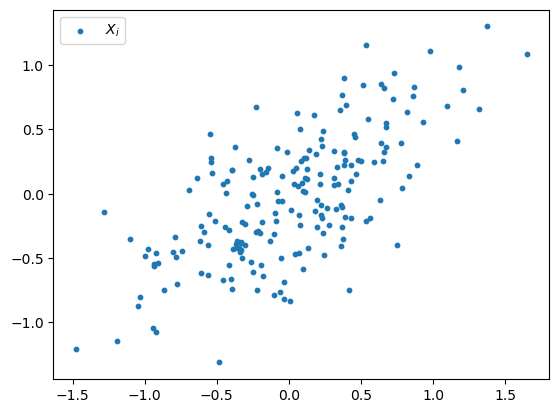
\includegraphics[width=.45\textwidth]{./Illustrations/pca_toy}
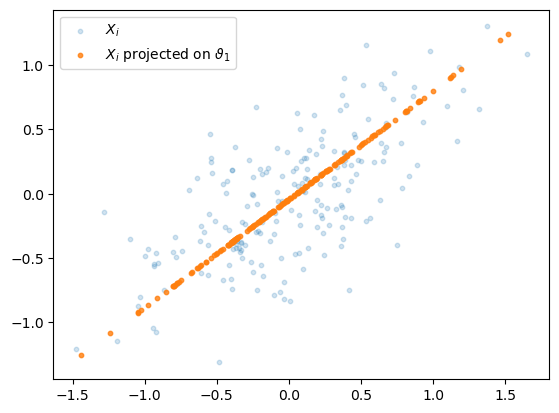
\includegraphics[width=.45\textwidth]{./Illustrations/pca_toy_proj}
        \caption{\small PCA on the first component of $(X_i)_{1\leq i \leq 200}$ i.i.d. Gaussian random variables in $\rset^2$. The first vector $\vartheta_1$ provides 46\% of the explained variance. (Right) The coordinate of $X_i$ along $\vartheta$ is given by $c_1(i)$ (orange dots).} 
        \label{fig:pca:toy}
    \end{figure*}

\section{PCA visualization}
Using Scikit-learn  (\url{https://scikit-learn.org/}) we can display comprehensive visualizations of dimensionality reduction with PCA. For a simple illustration we use the Iris dataset\footnote{\url{https://scikit-learn.org/1.5/auto_examples/datasets/plot_iris_dataset.html}} in which $n=150$ and each $X_i$, $1\leqslant i \leqslant n$, is the observation of an iris (Setosa, Versicolour, or Virginica) described by $d=4$ features: Sepal Length, Sepal Width, Petal Length and Petal Width. Figure~\ref{fig:pca:iris} displays the dataset and Figure~\ref{fig:pca:iris:proj} the result of a PCA on the 4 components. The two first components provide 97.8\% of the explained variance. The illustrations are obtained following \url{https://plotly.com/python/pca-visualization/}.

\begin{figure*}
        \centering
            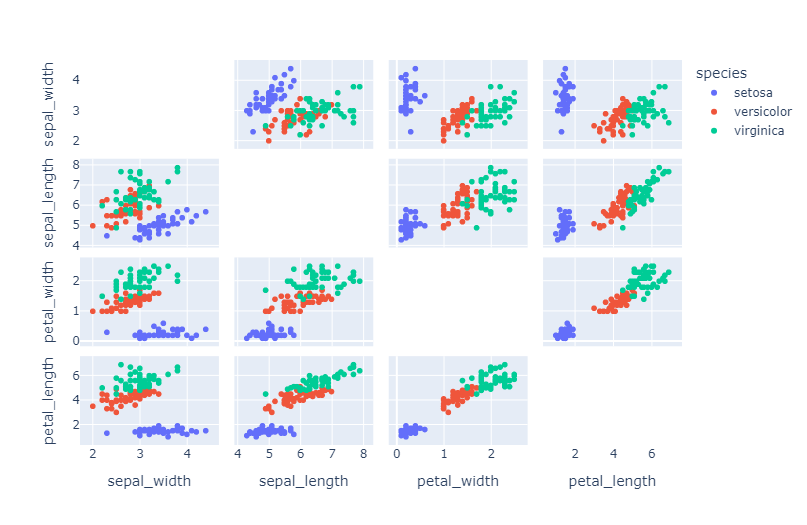
\includegraphics[width=.9\textwidth]{./Illustrations/pca_iris}
        \caption{\small Iris dataset.} 
        \label{fig:pca:iris}
    \end{figure*}

\begin{figure*}
        \centering
            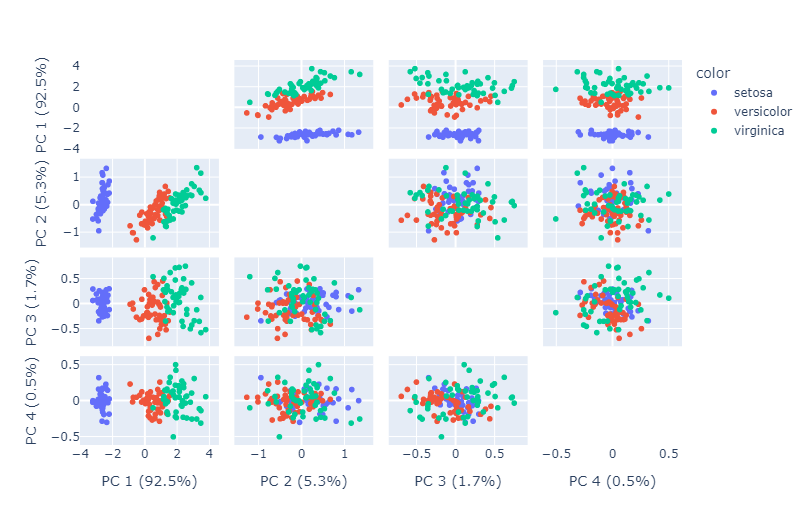
\includegraphics[width=.9\textwidth]{./Illustrations/pca_iris_proj}
        \caption{\small PCA on the four components of the iris dataset. The graph in row $i$ and column $j$ displays the projection of each $X_i$ on the subspace generated by $\{\vartheta_i,\vartheta_j\}$ i.e. the two dimensional projection related to principal components $c_i$ and $c_j$. Illustration from \url{https://scikit-learn.org/1.5/auto_examples/datasets/plot_iris_dataset.html}.} 
        \label{fig:pca:iris:proj}
    \end{figure*}

%\paragraph{{\bf Projection quality - variables}}
%To be detailed.
%Let $1\leqslant k \leqslant d$ and consider the variable $X_{.k}$, the $k$-th column of $X$ and $D   = \mathrm{diag}(n^{-1},\ldots,n^{-1})$. $\langle a, b\rangle_D = a'Db$. 
%\[ 
%\rho_k(j) = \frac{\langle X_{.k}, v_j\rangle_D}{\|X_{.k}\|_D\|v_j\|_{D}}\eqsp,
%\]
%Let $W_p = \mathrm{span}\{v_1,\ldots,v_p\}$. Note that for all $1 \le i \le K$,
%\[
%\|\rho_k\|_D^2 = \frac{\|\pi_{W_Q}(X_{.k})\|_D^2}{\|X_{.k}\|_D^2}\le 1\eqsp. 
%\] 
%$\|\rho_k\|$ measures the quality of the projection of $X_{.k}$ on the first $Q$ principal components. When the variables are scaled, $\|X_{.k}\|_D^2=1$ the cos^2 for a variable corresponds to its coordinate squared: $(\langle X_{.k}, v_j\rangle_D)^2$.
%The quality of projection can also be defined for the individuals.

%\includepdf[pages=-]{./Data/pca.pdf}
